\hypertarget{hexl_8hpp}{}\section{hexl.\+hpp File Reference}
\label{hexl_8hpp}\index{hexl.\+hpp@{hexl.\+hpp}}
{\ttfamily \#include \char`\"{}hexl/eltwise/eltwise-\/add-\/mod.\+hpp\char`\"{}}\newline
{\ttfamily \#include \char`\"{}hexl/eltwise/eltwise-\/cmp-\/add.\+hpp\char`\"{}}\newline
{\ttfamily \#include \char`\"{}hexl/eltwise/eltwise-\/cmp-\/sub-\/mod.\+hpp\char`\"{}}\newline
{\ttfamily \#include \char`\"{}hexl/eltwise/eltwise-\/fma-\/mod.\+hpp\char`\"{}}\newline
{\ttfamily \#include \char`\"{}hexl/eltwise/eltwise-\/mult-\/mod.\+hpp\char`\"{}}\newline
{\ttfamily \#include \char`\"{}hexl/eltwise/eltwise-\/reduce-\/mod.\+hpp\char`\"{}}\newline
{\ttfamily \#include \char`\"{}hexl/eltwise/eltwise-\/sub-\/mod.\+hpp\char`\"{}}\newline
{\ttfamily \#include \char`\"{}hexl/ntt/ntt.\+hpp\char`\"{}}\newline
{\ttfamily \#include \char`\"{}hexl/util/util.\+hpp\char`\"{}}\newline
Include dependency graph for hexl.\+hpp\+:
\nopagebreak
\begin{figure}[H]
\begin{center}
\leavevmode
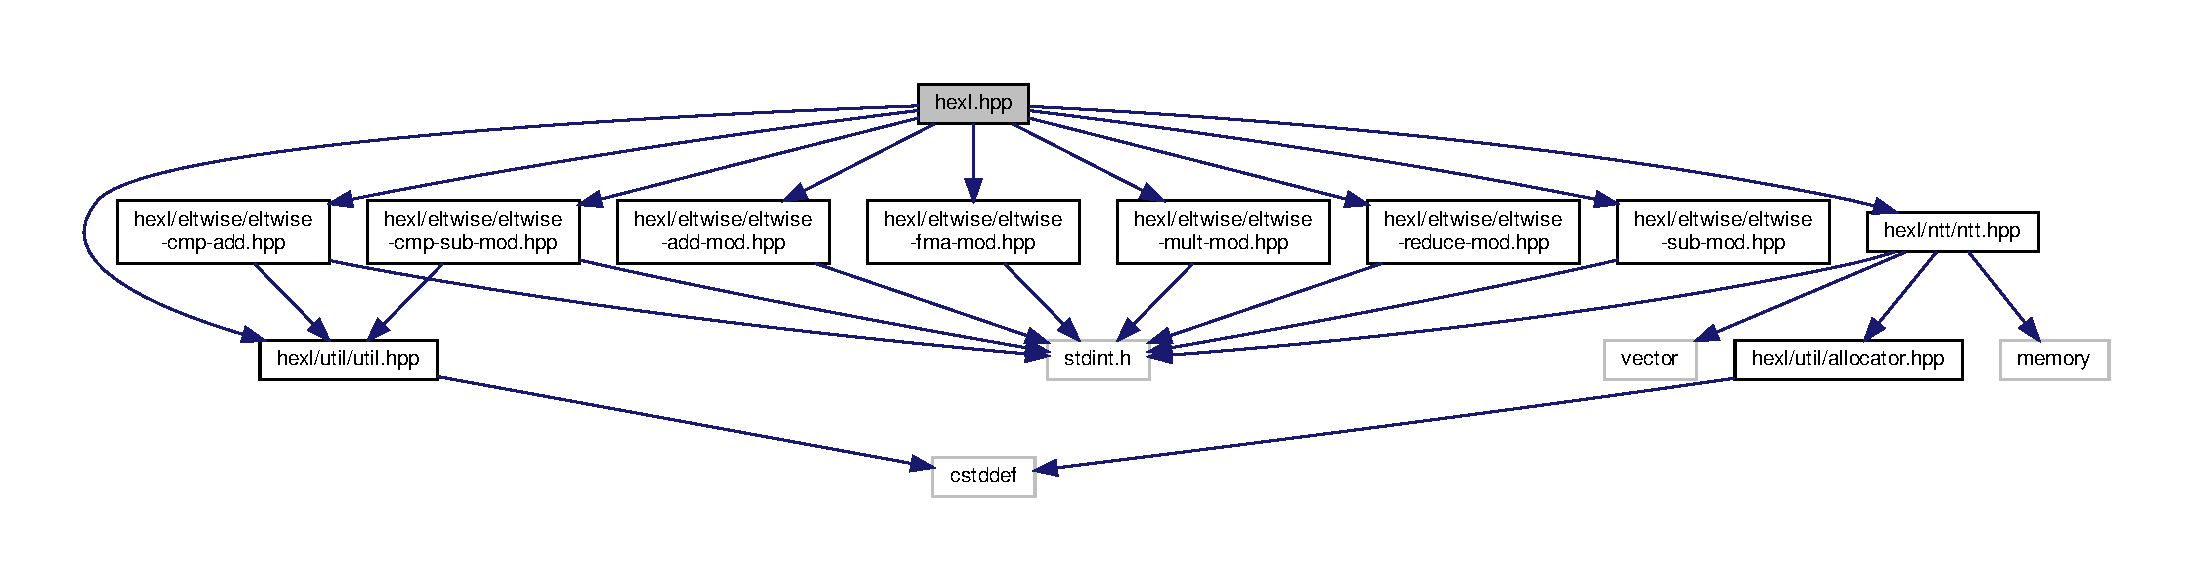
\includegraphics[width=350pt]{hexl_8hpp__incl}
\end{center}
\end{figure}
